\begin{frame}{Feature Branches (1)}
\begin{columns}[T]
  \begin{column}{.45\textwidth}
    \begin{block}{}
      \includegraphics[scale=0.6]{images/feature-branches1.png}
    \end{block}
  \end{column}
  \begin{column}{.1\textwidth}
    \begin{block}{}
      \pause $\longrightarrow$
    \end{block}
  \end{column}
  \begin{column}{.45\textwidth}
    \begin{block}{}  
        \pause \includegraphics[scale=0.6]{images/feature-branches2.png}
    \end{block}
  \end{column}
\end{columns}  
\begin{tiny}
\pause \texttt{git merge dumbidea} \\
\pause \texttt{git merge iss91v2} \\
\pause \texttt{git branch -D iss91} \\
\end{tiny}
\end{frame}

\begin{frame}{Long-Running Branches}
\begin{figure} 
\centering
  \includegraphics[scale=0.5]{images/long-running-branch.pdf}
\end{figure}
\begin{tiny}
\pause @branch \\
\pause \texttt{git add ...} \\
\pause \texttt{git commit} \\
\end{tiny}
\end{frame}

\begin{frame}{Long-Running Branches}
\begin{figure} 
\centering
  \includegraphics[scale=0.5]{images/long-running-branch2.pdf}
\end{figure}
\begin{tiny}
\pause @master \\
\pause \texttt{git add ...} \\
\pause \texttt{git commit} \\
\end{tiny}

\end{frame}

\begin{frame}{Long-Running Branches}
\begin{figure} 
\centering
  \includegraphics[scale=0.4]{images/long-running-branch3.pdf}
\end{figure}
\begin{tiny}
\pause @branch \\
\pause \texttt{git rebase master} \\
\end{tiny}

\end{frame}


\begin{frame}{Zentralisierter Workflow}
\begin{figure} 
\centering
\includegraphics[scale=0.6]{images/centralized-workflow.pdf}
\end{figure}
\begin{itemize}
\pause \item Bekannt aus SVN
\pause \item Git verhindert überschreiben von Daten
\end{itemize}
\end{frame}

\begin{frame}{Integration-Manager Workflow}
\begin{figure} 
\centering
\includegraphics[scale=0.6]{images/integration-manager-workflow.pdf}
\begin{itemize}
\pause \item The project maintainer pushes to their public repository.
\pause \item A contributor clones that repository and makes changes.
\pause \item The contributor pushes to their own public copy.
\pause \item The contributor sends the maintainer an e-mail asking them to pull changes.
\pause \item The maintainer adds the contributor’s repo as a remote and merges locally.
\pause \item The maintainer pushes merged changes to the main repository.
\end{itemize}
\end{figure}
\end{frame}

\begin{frame}{Dictator and Lieutenant Workflow}
\begin{figure} 
\centering
\includegraphics[scale=0.3]{images/dictator-and-lieteutnant-workflow.pdf}
\begin{itemize}
\pause \item Regular developers work on their topic branch and rebase their work on top of master. The master branch is that of the dictator.
\pause \item Lieutenants merge the developers’ topic branches into their master branch.
\pause \item The dictator merges the lieutenants’ master branches into the dictator’s master branch.
\pause \item The dictator pushes their master to the reference repository so the other developers can rebase on it.
\end{itemize}
\end{figure}
\end{frame}